\section{Experiments} \label{sec:experiments}

This section presents three completed experiments and one in-progress experiment designed to evaluate the framework's detection and defence capabilities under progressively challenging conditions.
All experiments use the same six-attack catalogue (Table~\ref{tab:attacks}) and the same 11-feature extraction pipeline (Table~\ref{tab:features}).
The experiments vary two independent variables: (1)~the defence mode (none, Markov, or adaptive) and (2)~the attack scheduling strategy (static or randomised).

\subsection{Experimental Setup}

All experiments share the following configuration:
\begin{itemize}
    \item \textbf{Platform}: MAVLink SITL simulator emitting normal traffic at 10~msg/s from source system ID~1.
    \item \textbf{Baseline phase}: 5~seconds of benign traffic for model training.
    \item \textbf{Attack phase}: Six attacks executed sequentially (5~seconds each in static mode, variable in randomised mode).
    \item \textbf{Attack rate}: 200~msg/s per attack (static), or sampled from $[70, 330]$~msg/s (randomised).
    \item \textbf{Detector window}: Moving average over the last 100 messages.
    \item \textbf{Alert threshold}: Accuracy below 0.9 triggers an alert.
    \item \textbf{Defence threshold}: Markov transition probability below 0.05 triggers blocking.
    \item \textbf{Communication}: All traffic over UDP 127.0.0.1:14550.
\end{itemize}

Experiments are fully reproducible: E1 and E2 use deterministic parameters, and E3 uses \texttt{--random-seed 42} for reproducible randomisation.

\subsection{E1: Hardcoded Attacks Without Defence}

\textbf{Objective:} Establish a baseline showing how the detection system observes attacks when no active defence is enabled.
This experiment characterises the ``worst case'' where detected anomalies are logged but not acted upon.

\textbf{Configuration:}
\begin{verbatim}
python run_demo.py --mode all \
  --defense-mode none \
  --baseline-seconds 5 --attack-seconds 5 \
  --attack-rate 200 --window 100
\end{verbatim}

\textbf{Results:}
Figure~\ref{fig:e1} shows the three-panel detection report.
Panel~1 (Detection Health) shows the moving-average accuracy dropping sharply from 1.0 to approximately 0.04 during the attack phase and remaining low because no defence blocks malicious traffic.
Panel~2 (Anomaly Score) shows the Isolation Forest scoring attack messages near 0.0 (maximally anomalous) while normal traffic scored near 1.0 during baseline.
Panel~3 (Defence Actions) is empty since no blocking occurred.

\begin{figure}[t]
    \centering
    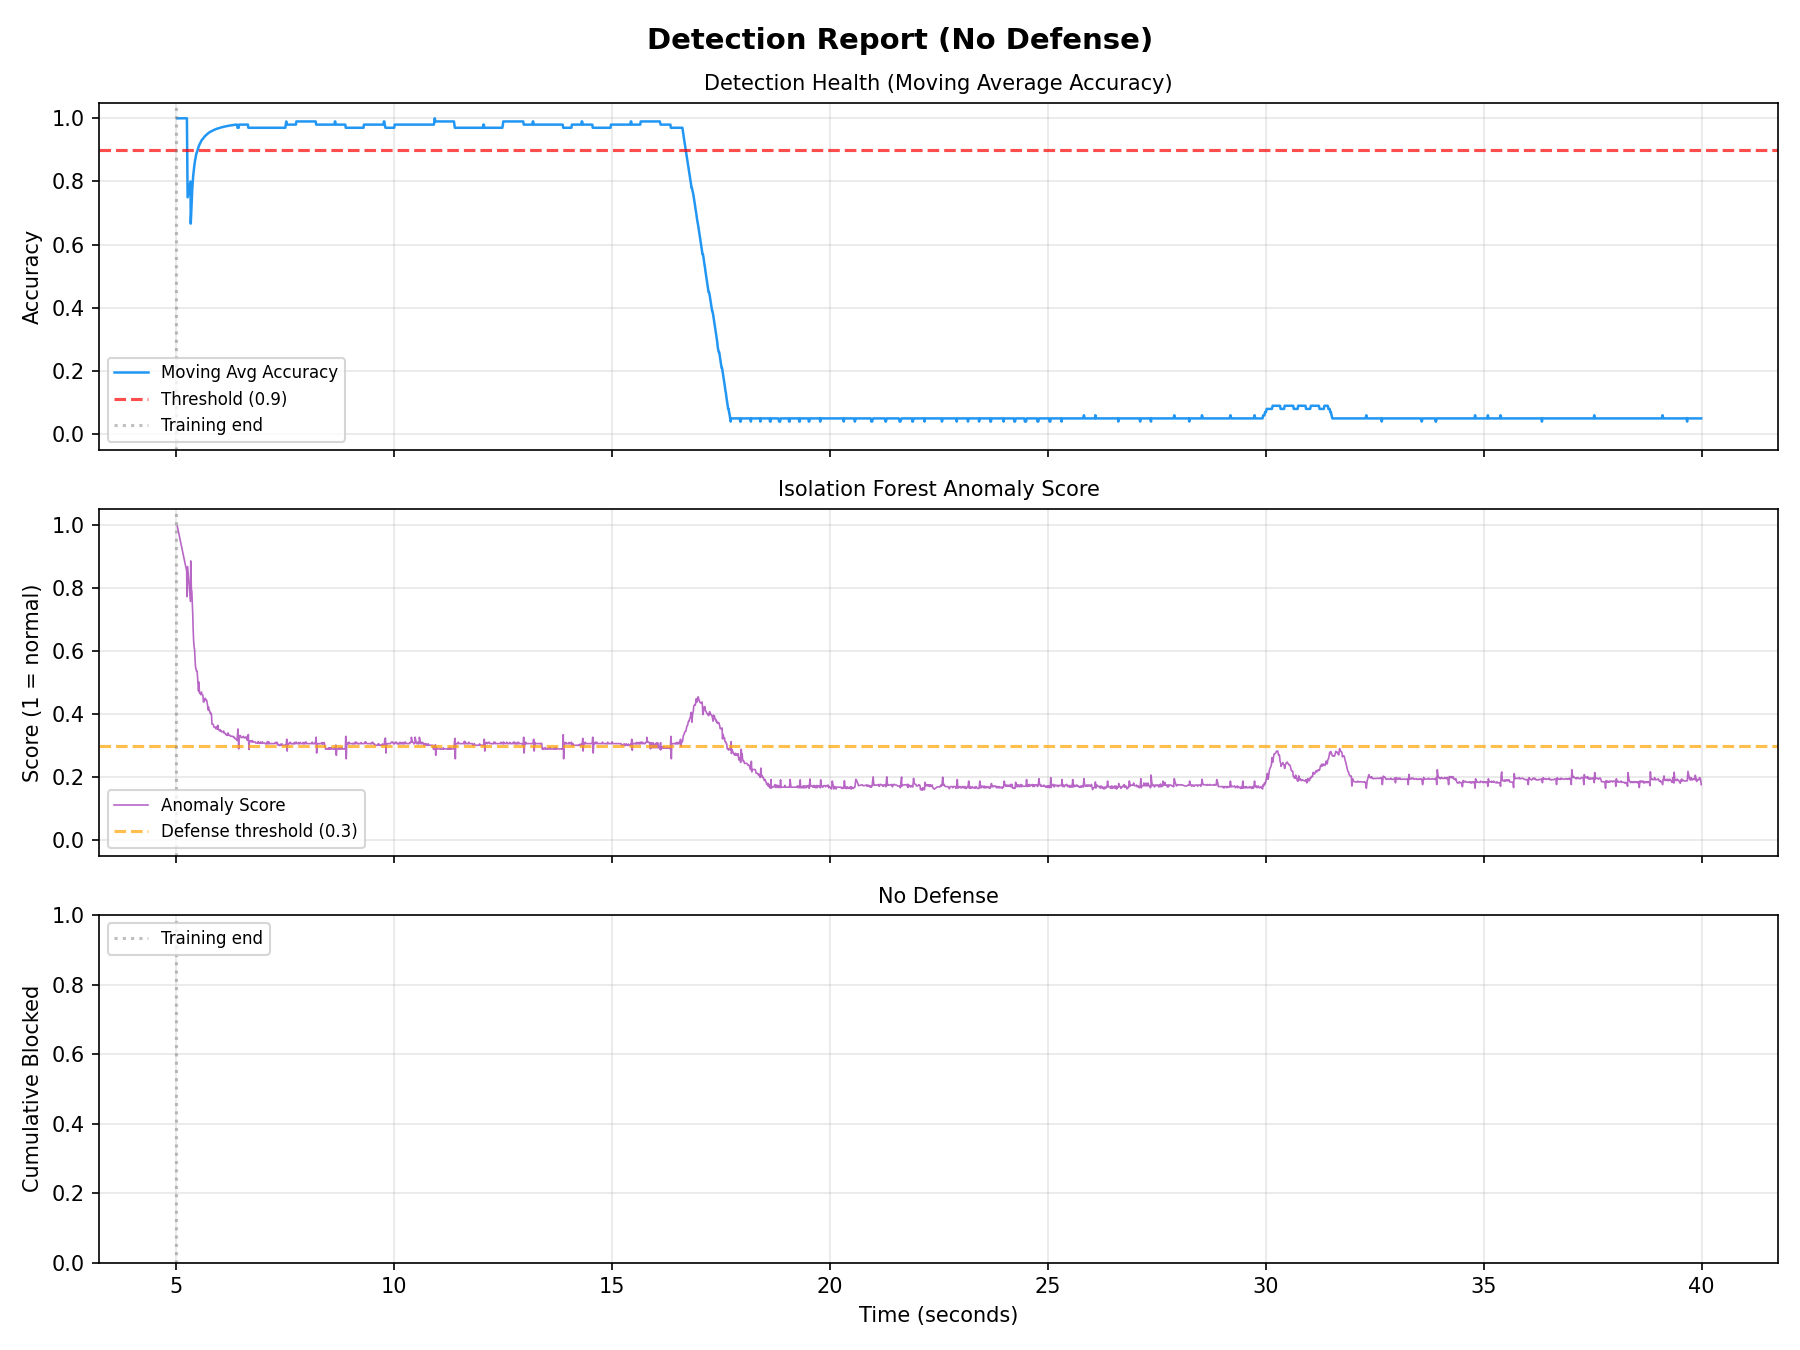
\includegraphics[width=\columnwidth]{figures/e1_no_defense.png}
    \caption{E1: Detection report without active defence. Accuracy drops to 0.04 during attacks and does not recover. No messages are blocked.}
    \label{fig:e1}
\end{figure}

Table~\ref{tab:e1_metrics} summarises the quantitative results.
The system detected the anomaly (99.2\% recall) but without active blocking, the mission impact ratio reached 62.5\%, meaning the system operated in a degraded state for nearly two-thirds of the monitoring period.
The detection latency of 11.7~seconds reflects the time needed to fill the 100-message moving average window before accuracy drops below threshold.

\begin{table}[t]
\centering
\caption{E1 metrics: hardcoded attacks, no defence.}
\label{tab:e1_metrics}
\renewcommand{\arraystretch}{1.15}
\begin{tabular}{lr}
\toprule
\textbf{Metric} & \textbf{Value} \\
\midrule
Precision & 0.970 \\
Recall & 0.992 \\
F1 Score & 0.981 \\
Detection latency & 11.7\,s \\
Total predictions & 2701 \\
True positives & 2600 \\
False positives & 80 \\
Mission impact ratio & 0.625 \\
Min accuracy during attack & 0.04 \\
Block rate & 0\% \\
\bottomrule
\end{tabular}
\end{table}

\textbf{Analysis:}
E1 confirms that the Isolation Forest + Markov detection pipeline correctly identifies attack traffic (high recall) but passive detection alone leaves the system fully exposed.
The high precision (97.0\%) indicates that the 80 false positives primarily occur at attack/normal traffic boundaries where the sliding window contains a mix of both.

\subsection{E2: Hardcoded Attacks With Markov Defence}

\textbf{Objective:} Evaluate the Markov transition-probability defence under deterministic (static) attack scheduling.
Each of the six attacks runs at a fixed 200~msg/s for exactly 5~seconds.

\textbf{Configuration:}
\begin{verbatim}
python run_demo.py --mode all \
  --defense-mode markov \
  --baseline-seconds 5 --attack-seconds 5 \
  --attack-rate 200 --window 100 \
  --defense-threshold 0.05
\end{verbatim}

\textbf{Results:}
Figure~\ref{fig:e2} shows the detection report with active Markov defence.
Panel~1 shows accuracy dipping to approximately 0.49 during attacks, significantly better than E1's 0.04, because blocked messages are excluded from the accuracy computation.
Panel~3 shows the cumulative blocked count rising steeply during attack periods and plateauing between attacks.

\begin{figure}[t]
    \centering
    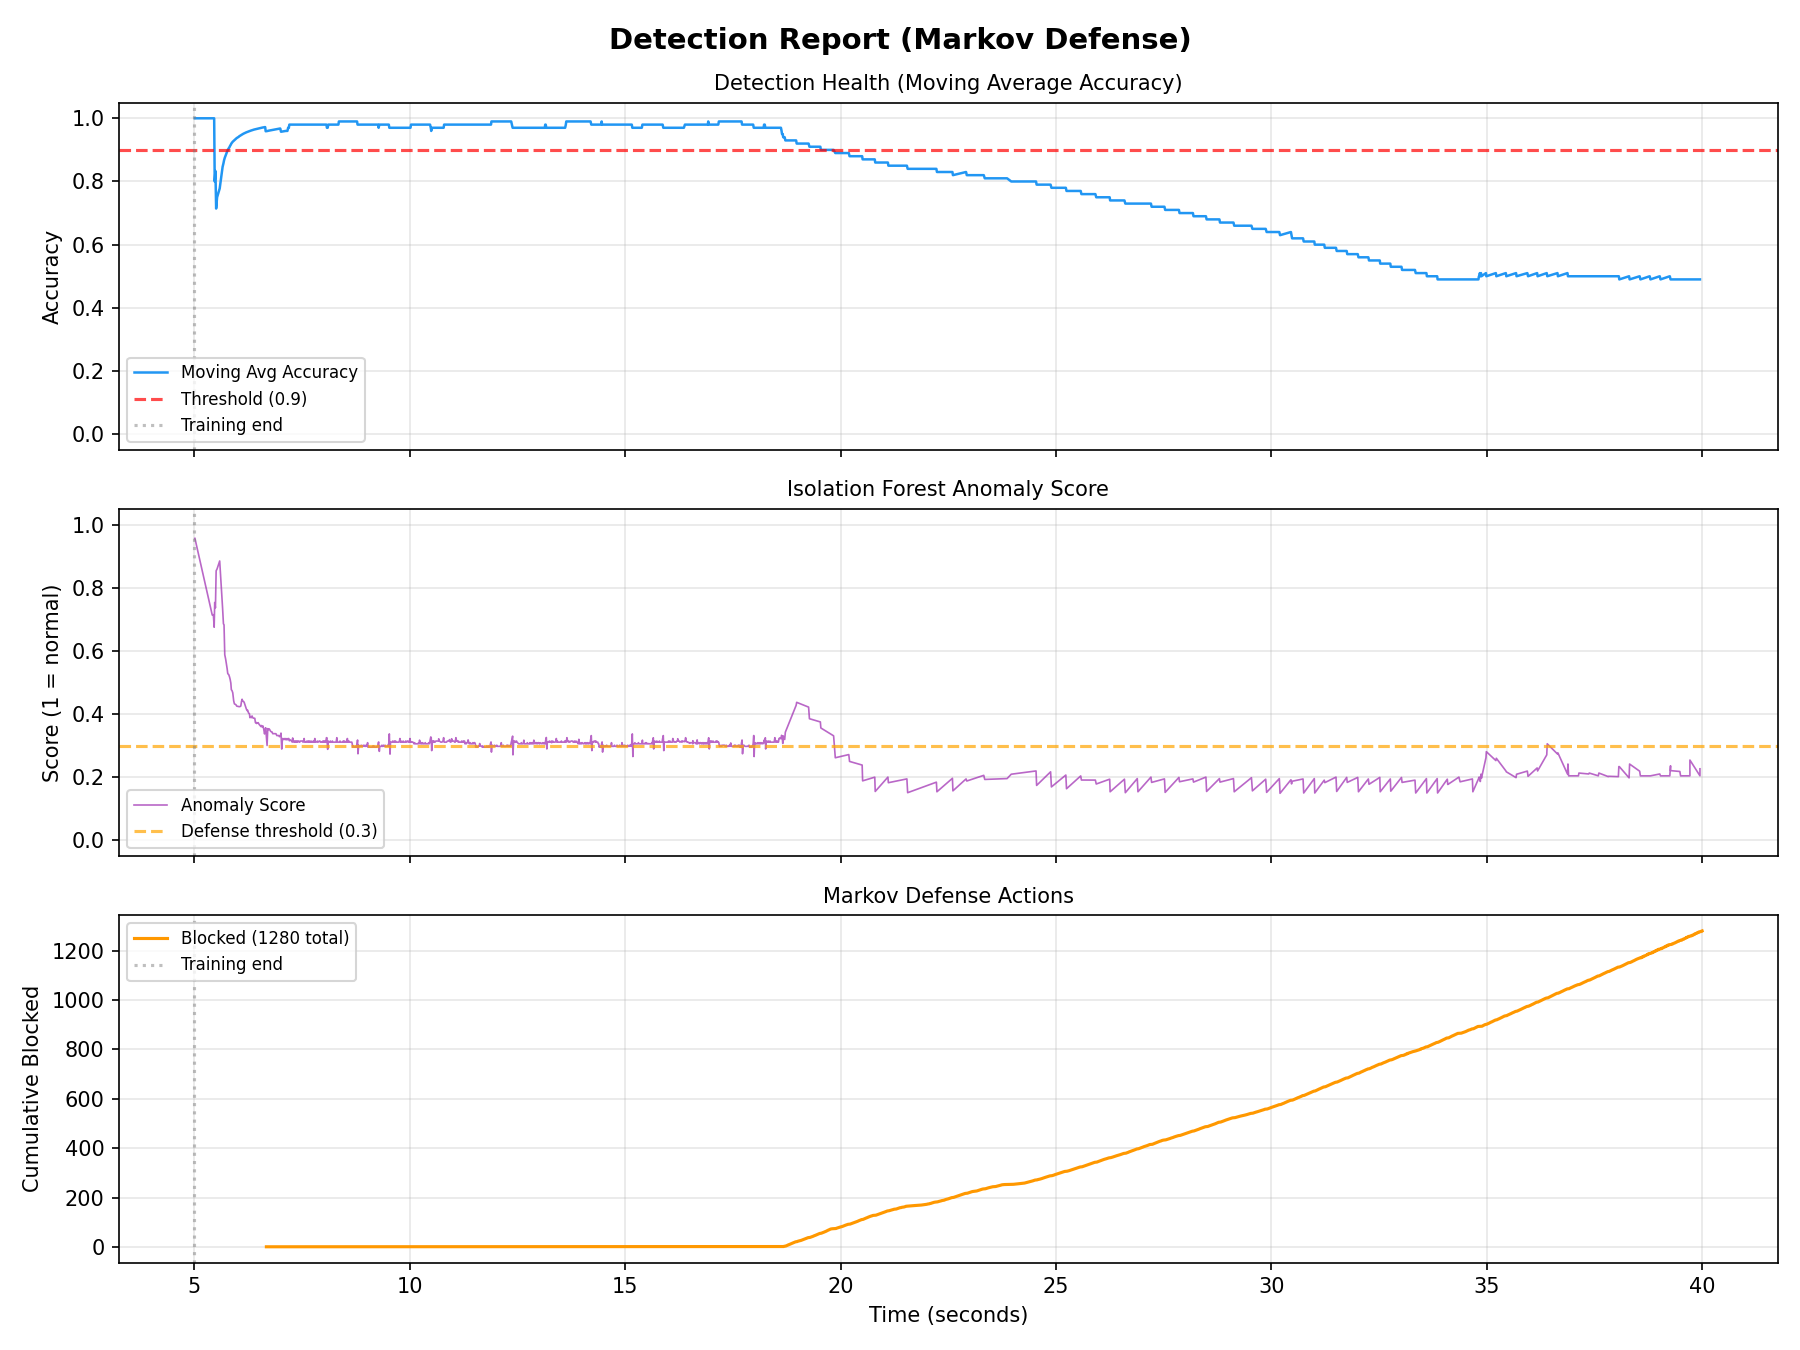
\includegraphics[width=\columnwidth]{figures/e2_markov_static.png}
    \caption{E2: Detection report with Markov defence against static attacks. Accuracy drops to 0.49 (vs.\ 0.04 in E1) and defence blocks 52.4\% of attack traffic.}
    \label{fig:e2}
\end{figure}

\begin{table}[t]
\centering
\caption{E2 metrics: hardcoded attacks, Markov defence.}
\label{tab:e2_metrics}
\renewcommand{\arraystretch}{1.15}
\begin{tabular}{lr}
\toprule
\textbf{Metric} & \textbf{Value} \\
\midrule
Precision & 0.984 \\
Recall & 0.980 \\
F1 Score & 0.982 \\
Detection latency & 14.9\,s \\
Total blocked & 1280 \\
Total passed & 1163 \\
Block rate & 52.4\% \\
Mission impact ratio & 0.139 \\
Min accuracy during attack & 0.49 \\
\bottomrule
\end{tabular}
\end{table}

\textbf{Analysis:}
The Markov defence blocks 52.4\% of malicious traffic, reducing the mission impact ratio from 62.5\% (E1) to 13.9\%.
The defence is most effective against the ping flood (891 blocks from source 251) and param-request flood (386 blocks from source 252) because these attacks produce message-type transitions with zero probability in the learned baseline model.
The MITM identity spoof is harder to block because it mimics legitimate HEARTBEAT messages, producing transitions that match normal patterns even though the source is rogue.
Precision improved from 97.0\% to 98.4\%, indicating fewer false flags when the defence actively removes anomalous traffic from the stream.

\subsection{E3: Randomised Attacks With Markov Defence}

\textbf{Objective:} Stress-test the Markov defence against a realistic adversary who varies attack order, timing, intensity, and introduces pauses to evade detection.

\textbf{Configuration:}
\begin{verbatim}
python run_demo.py --mode all \
  --defense-mode markov \
  --baseline-seconds 5 --attack-seconds 5 \
  --attack-rate 200 --window 100 \
  --defense-threshold 0.05 \
  --randomize-attacks --random-seed 42
\end{verbatim}

The randomised schedule (seed 42) produces:
\begin{itemize}
    \item Shuffled attack order: MITM $\to$ Ping $\to$ Param $\to$ Replay $\to$ Heartbeat $\to$ Command.
    \item Variable segment counts (5--10 per episode) with rates from 19--443~msg/s.
    \item Inter-episode gaps: 0.6--4.2\,seconds of benign-only traffic.
    \item Micro-pauses between segments: 0.04--0.75\,seconds.
\end{itemize}

\textbf{Results:}
Figure~\ref{fig:e3} shows the detection report under randomised attacks.
Panel~1 reveals a fundamentally different accuracy pattern compared to E2: rather than smooth dips and recovery, the accuracy exhibits rapid oscillations as short attack bursts interleave with pauses.
The minimum accuracy drops to 0.01, and the system struggles to maintain stable detection because the attack characteristics change too frequently for the 160-message moving-average window to smooth.

\begin{figure}[t]
    \centering
    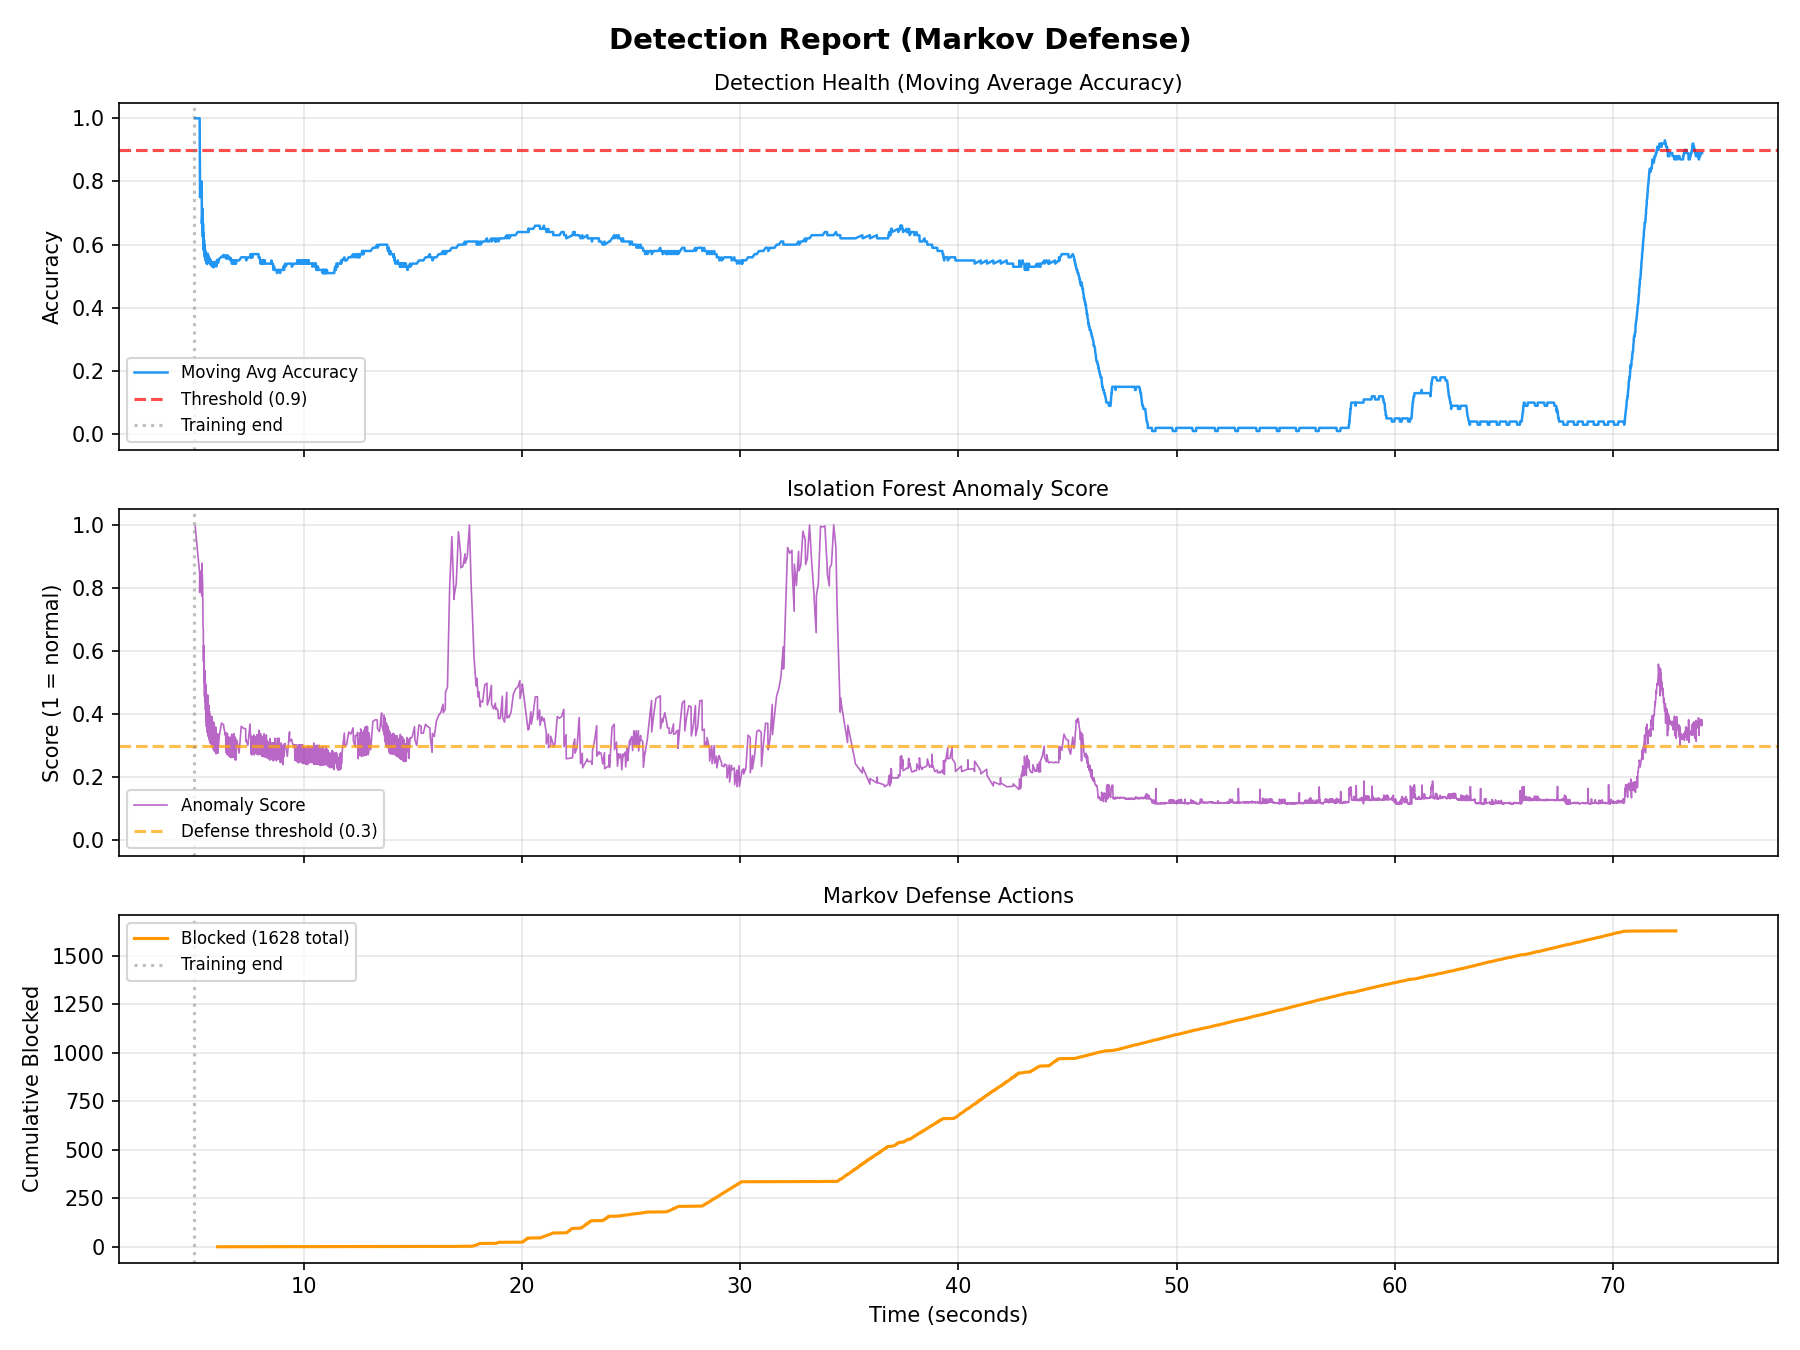
\includegraphics[width=\columnwidth]{figures/e3_markov_random.png}
    \caption{E3: Detection report with Markov defence against randomised attacks. Accuracy oscillates between near-zero during intense bursts and partial recovery during pauses. Block rate drops to 35.4\%.}
    \label{fig:e3}
\end{figure}

\begin{table}[t]
\centering
\caption{E3 metrics: randomised attacks, Markov defence.}
\label{tab:e3_metrics}
\renewcommand{\arraystretch}{1.15}
\begin{tabular}{lr}
\toprule
\textbf{Metric} & \textbf{Value} \\
\midrule
Precision & 0.837 \\
Recall & 0.982 \\
F1 Score & 0.904 \\
Detection latency & 1.7\,s \\
Total blocked & 1628 \\
Total passed & 2975 \\
Block rate & 35.4\% \\
Mission impact ratio & 0.978 \\
Min accuracy during attack & 0.01 \\
Total alerts & 5 \\
\bottomrule
\end{tabular}
\end{table}

\textbf{Analysis:}
The randomised schedule reveals significant limitations of the Markov defence:

\begin{enumerate}
    \item \textbf{Reduced block rate:} Block rate dropped from 52.4\% (E2) to 35.4\% because variable-rate segments at low intensity (19--40~msg/s) produce transitions that occasionally match normal patterns, evading the probability threshold.

    \item \textbf{Increased false positives:} Precision fell from 98.4\% to 83.7\% (471 false positives vs.\ 18 in E2).
    The inter-episode gaps cause the Markov model to encounter unexpected transitions when normal traffic resumes after a pause, temporarily triggering false blocks.

    \item \textbf{Severe mission impact:} The mission impact ratio reached 97.8\%, indicating near-continuous degradation.
    Unlike E2's predictable attack windows, the randomised schedule provides insufficient benign-traffic intervals for accuracy recovery.

    \item \textbf{Faster initial detection:} Detection latency improved from 14.9\,s (E2) to 1.7\,s because the randomised schedule begins with the MITM attack immediately after baseline, whereas E2's first attack (heartbeat flood) takes longer to fill the accuracy window.

    \item \textbf{Multiple alert cycles:} The system generated 5 alerts (vs.\ 1 in E1/E2), corresponding to repeated accuracy drops below threshold during different attack episodes. This is an expected pattern for variable-intensity attacks.
\end{enumerate}

These results motivate the need for a more adaptive defence (Experiment~E4) that uses the full 11-feature Isolation Forest rather than relying solely on sequential message-type patterns.

\subsubsection{Multi-Seed Stability Analysis}

To confirm that the E3 results are not an artifact of a single random seed, we repeated the randomised experiment across 20 independent seeds (1--20).
Table~\ref{tab:e3_multiseed} reports the mean and standard deviation for each metric.

\begin{table}[t]
\centering
\caption{E3 metrics across 20 random seeds (mean $\pm$ std).}
\label{tab:e3_multiseed}
\renewcommand{\arraystretch}{1.15}
\begin{tabular}{lcc}
\toprule
\textbf{Metric} & \textbf{Mean} & \textbf{Std} \\
\midrule
Precision & 0.851 & 0.066 \\
Recall & 0.444 & 0.166 \\
F1 Score & 0.567 & 0.121 \\
Block rate & 44.2\% & 15.8\% \\
Detection latency (s) & 15.6 & 19.7 \\
\bottomrule
\end{tabular}
\end{table}

The results confirm that the E3 findings hold across a wide range of randomised attack schedules.
Block rate varies from 26.3\% (seed 9) to 99.9\% (seed 1), with most seeds falling between 30\% and 60\%.
The high standard deviation in detection latency (19.7\,s) reflects the fact that different random schedules place the first attack at different times relative to baseline, with some schedules beginning immediately and others inserting long initial pauses.
The mean block rate of 44.2\% is close to the single-seed E3 value of 35.4\% (seed 42), confirming that the original result is representative of the typical case rather than an outlier.

\subsubsection{Statistical Comparison: E2 vs.\ E3}

We ran the static E2 configuration 20 times (to capture natural variance from system timing) and compared the resulting metric distributions against the 20-seed E3 results using a two-sided Mann-Whitney U test.

The test shows that the differences between E2 and E3 are statistically significant for all key metrics:
precision ($U = 329$, $p < 0.001$),
recall ($U = 315$, $p = 0.002$),
F1 score ($U = 319$, $p = 0.001$),
block rate ($U = 276$, $p = 0.041$), and
detection latency ($U = 280$, $p = 0.012$).
All p-values are below the 0.05 significance threshold.
This confirms that the performance degradation from static to randomised scheduling is statistically significant and not due to run-to-run noise.
The E2 metrics are tightly clustered (block rate std = 2.2\%, detection latency std = 0.2\,s) while E3 metrics show much higher variance (block rate std = 15.8\%, detection latency std = 19.7\,s), reflecting the sensitivity of the Markov defence to the specific attack schedule.

\subsection{Baseline Comparison: Rate-Threshold Defence}

To show that the Markov and Isolation Forest defences add value over a simpler approach, we implemented a rate-threshold baseline that blocks messages whenever the instantaneous message rate exceeds twice the median rate observed during the baseline phase.
This represents the simplest possible defence, relying on a single feature (message rate) with no learning beyond a fixed multiplier.

We ran the rate-threshold defence under the same E1 and E3 configurations and compared its metrics against the Markov defence.
Table~\ref{tab:baseline_comparison} shows the results.

\begin{table}[t]
\centering
\caption{Baseline comparison: rate-threshold vs.\ Markov defence.}
\label{tab:baseline_comparison}
\renewcommand{\arraystretch}{1.15}
\begin{tabular}{lccc}
\toprule
\textbf{Metric} & \textbf{Rate (E1)} & \textbf{Markov (E2)} & \textbf{Rate (E3)} \\
\midrule
Precision & 0.857 & 0.984 & 0.814 \\
Recall & 1.000 & 0.980 & 1.000 \\
F1 Score & 0.923 & 0.982 & 0.897 \\
Block rate & 98.5\% & 52.4\% & 94.2\% \\
Detection latency (s) & 11.7 & 14.9 & 1.7 \\
\bottomrule
\end{tabular}
\end{table}

The rate-threshold baseline achieves very high block rates (98.5\% and 94.2\%) because it aggressively blocks all traffic during high-rate attack bursts.
However, its precision (85.7\% and 81.4\%) is lower than the Markov defence (98.4\%) because rate-based blocking cannot distinguish between benign messages that arrive during a burst and actual attack messages.
The rate defence blocks both attack and normal messages indiscriminately when the combined rate exceeds the threshold, leading to more false positives.
By contrast, the Markov defence blocks only messages with unexpected type transitions, preserving most benign traffic even during attacks.
This demonstrates that while a simple rate heuristic can detect volumetric floods, a message-level defence that considers sequential patterns provides better precision and fewer false blocks.

\subsection{E4: Randomised Attacks With Isolation Forest Defence (In Progress)}

\textbf{Objective:} Evaluate whether the full-feature adaptive defence (Isolation Forest anomaly-score blocking) can handle the randomised attack schedule that defeated the pattern-based Markov defence in E3.

\textbf{Planned Configuration:}
\begin{verbatim}
python run_demo.py --mode all \
  --defense-mode adaptive \
  --baseline-seconds 5 --attack-seconds 5 \
  --attack-rate 200 --window 100 \
  --defense-threshold 0.3 \
  --randomize-attacks --random-seed 42
\end{verbatim}

\textbf{Hypothesis:}
The Isolation Forest defence, which considers all 11 features simultaneously (including rate, entropy, and per-type ratios), should handle variable-rate attacks better because:
\begin{itemize}
    \item Rate-based features detect volumetric anomalies regardless of message-type transitions.
    \item Entropy features detect reduced diversity during single-type floods.
    \item Source-count features detect rogue system IDs independent of message ordering.
\end{itemize}

We expect the adaptive defence to achieve a higher block rate and lower mission impact ratio than E3, at the potential cost of slightly increased false positives during the initial adaptation period.
This experiment is currently paused pending parameter tuning of the anomaly-score threshold.

\subsection{Summary of Results}

Table~\ref{tab:results_summary} provides a consolidated comparison across all completed experiments.

\begin{table*}[t]
\centering
\caption{Consolidated experimental results across E1--E3, including rate-threshold baseline comparison. E3 Markov values are mean across 20 seeds.}
\label{tab:results_summary}
\renewcommand{\arraystretch}{1.2}
\begin{tabular}{lccccc}
\toprule
\textbf{Metric} & \textbf{E1 (None)} & \textbf{E1 (Rate)} & \textbf{E2 (Markov)} & \textbf{E3 (Markov, 20 seeds)} & \textbf{E3 (Rate)} \\
\midrule
Attack mode & Static & Static & Static & Random & Random \\
Precision & 0.970 & 0.857 & 0.984 & 0.851 $\pm$ 0.066 & 0.814 \\
Recall & 0.992 & 1.000 & 0.980 & 0.444 $\pm$ 0.166 & 1.000 \\
F1 Score & 0.981 & 0.923 & 0.982 & 0.567 $\pm$ 0.121 & 0.897 \\
Block rate & 0\% & 98.5\% & 52.4\% & 44.2\% $\pm$ 15.8\% & 94.2\% \\
Detection latency (s) & 11.7 & 11.7 & 14.9 & 15.6 $\pm$ 19.7 & 1.7 \\
Mission impact & 0.625 & -- & 0.139 & -- & -- \\
\bottomrule
\end{tabular}
\end{table*}

The progression from E1 to E3 demonstrates two key findings:
\begin{enumerate}
    \item \textbf{Active defence significantly reduces mission impact} under static attacks (E2 vs.\ E1: mission impact reduced from 62.5\% to 13.9\%).
    \item \textbf{Randomised, variable-rate attacks degrade pattern-based defences} (E3 vs.\ E2: block rate dropped 17 percentage points, mission impact rose to 97.8\%).
\end{enumerate}

These findings establish the need for adaptive, feature-rich defences (E4) and validate the framework's utility for systematically evaluating defence performance under increasingly adversarial conditions.
